\chapter{Evaluation}
...

\section{Dataset}
Our dataset consists on 12234 latex documents fetched from ArXiV. This documents correspond to the latest records harvested for CDS. The documents were processed using LateXML as described in the extraction process. From the given dataset, the simpler equations were filtered out (The ones containing one or two elements).


\section{Setup}

The machine used for experiments has a Intel Core i7 processor running at 3.4Ghz with 4 cores. The available RAM is 8Gb, and the Java Virtual Machine used for running Solr was run with the $-Xms2G -Xmx5G$ parameters. The complete specifications of the used software is presented in table \ref{sw_used}

\begin{longtable}{|m{2cm}|>
{\centering\arraybackslash}m{4cm}|>
{\centering\arraybackslash}m{4cm}|
}
\hline 
\textbf{Software} & 
\textbf{Version} 
\\
\hline
Operative System & Linux Mint 16 Petra (Ubuntu based) \\ \hline
Linux Kernel & 3.11.0-15 \\ \hline
Java Virtual Machine & 1.7.0-45 \\ \hline
Apache Solr & 4.6 \\ \hline
Python & 2.7.5+ \\ \hline
\caption{Software used during evaluations}
\label{sw_used}
\end{longtable}

\section{Results quality}
In this section we are interested in evaluating the quality of the results provided by our system.
The type of queries that MASE was designed for, are typical equations that can be found in a scientific publication. 
Out main user case is that a user of CDS is interested in finding documents inside the collection whose equations are related to the one that is provided.

\subsection{Equations}
The evaluated queries were provided by physics experts working at CERN from their own research topics. The queries were provided in \LaTeX format as the users used them in their own publications.
Table \ref{equations_table} presents the set of queries that were evaluated, and a simple explanation about it. 



\section{Comparison against other systems}
In this section we tried to compare our implementation of MASE(CDS) with the public available systems presented in the related work chapter. We judged if the fetched results of each system were relevant or not using the same criteria as for the previous section.  The systems were tested using Firefox 26.0
Table \ref{comparison_sw_table} presents the results of our test.

\begin{figure}
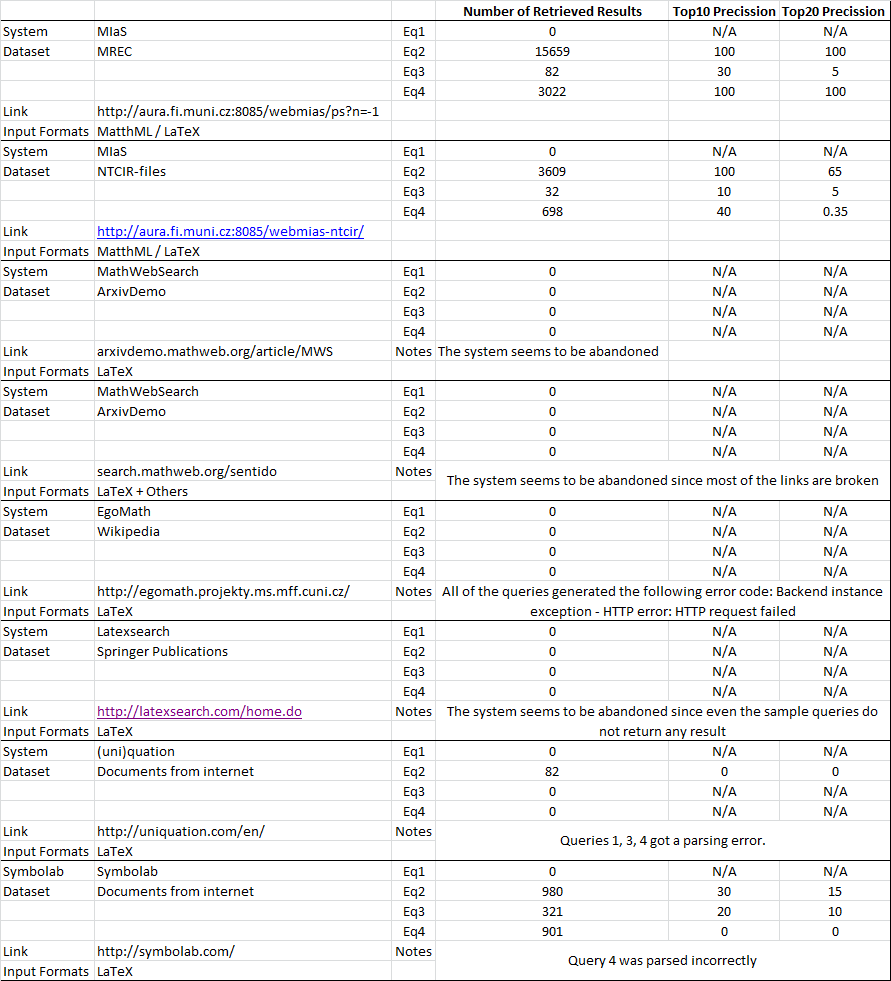
\includegraphics[height=15 cm]{figures/comparison_table.png}
\label{comparison_sw_table}
\caption{Results of comparison of available mathematical search systems}
\end{figure}

The results are a little disappointing since from the eight evaluated instances, only MIaS and Symbolab seem to be working properly. 

\section{Querying Performance}


\section{Indexing Performance}
For this set of evaluations, we were only interested in observing how the performance of the indexing stage is affected by the different types of features that are employed. We selected the first 100 records from our dataset and measured the total time it required to index all the elements in Solr using a python script and the solrpy library to do the communication. The default similarity in Solr was used. We also measured the index size at the end of each experiment.
Our four scenarios were organized as follows:
\begin{itemize}
\item N : Only notational features over the original expression were used
\item N+S : Notational and structural features over the original expression
\item N+S+NN : Notational and structural features over the original expression and notational features over the normalized string using Mathematica's Simplify function
\item N+S+FN : Notational and structural features over the original expression and notational features over the normalized string using Mathematica's Full Simplify function
\end{itemize}

Table \ref{indexing_performance} summarizes the results of this set of experiments. The first result is the significant increase in processing time when using Mathematica. Going from the N scenario to N+S represent an increase of almost 15x in the indexing time. Adding standard normalization increases the indexing time by a factor near to 1.44x and full normalization by a factor of 1.55x.

With respect to storage size, we see a small footprint (Less than 5\%)in the total size by going from N to N+S. Adding normalization represents an increase by a factor of 1.78x and the size of the fully normalized index represents a smaller increase (1.76x)

We can observe that there is a small trade-off between time and storage size depending on which normalization mode is employed.

\begin{longtable}{|c|c|p{2cm}|p{2cm}|p{2cm}|}
\hline 
Feature Set & Total time (sec) & Index Size (kb) & Avg. time per equation & Avg. size of equation (kb) \\ 
\hline 
N & 58 & 13926 & 0.00524 & 1.237 \\ 
\hline 
N+S & 884 & 14438 & 0.0785 & 1.282 \\ 
\hline 
N+S+NN & 1273 & 25780 & 0.113 & 2.345 \\ 
\hline 
N+S+FN & 1377 & 25548 & 0.122 & 2.269 \\ 
\hline
\caption{Indexing performance}
\label{indexing_performance}
\end{longtable} 

















